\documentclass{tufte-handout}

\usepackage{/Users/paulallen/OU/Astronomy/style}

\begin{document}
\tma{04}

\begin{question}

\qpart

Figure(a) This is the younger cluster.
\begin{itemize}
\item There is a dense central cluster of stars which indicate recent star formation.
\item There is a surrounding void possibly cleared by strong stellar winds or supernovae from massive young stars.
\item The presence of bright filament like structures facing the inner cluster are likely super heated interstellar
gas, now emitting in the visible and IR spectrum. 
\end{itemize}

\vspace{5cm}

Figure(b) The older cluster
\begin{itemize}
\item A large bright cluster without any obvious void suggesting the cluster has evolved over a longer period of time.
\item The absence of any interselar material also indicates that the orginal giant molecular cloud (GMC) has been fully 
consumed by star formation or dispersed by stellar feedback.
\item The interstellar filaments are now absent possibly due to secondary star formation.
\end{itemize}

\clearpage

\qpart

\begin{align*}
    T &\approx \frac{GMm}{kR}\\[8pt]
\stext{Make M the subject}\\
    T &\approx \frac{GMm}{kR}\\[8pt]
    kRT &\approx GMm\\[8pt]
    M &\approx \frac{kRT}{Gm}\\[8pt]
\stext{Substituting \( T = \SI{1.7e7}{\kelvin} \) and \( R = \SI{2.3}{\Rs} \)}\\
    &\approx \frac{\num{1.38e{-23}} \times \SI{2.3}{\Rs} \times \num{1.7e{7}}}{\num{6.67e{-11}} \times \frac{1}{2}\rb{\num{1.67e{-27}}}}\\[8pt]
    &\approx \num{6.742994012e{30}}\\[8pt]
\stext{divide by \unit{\Ms}}\\
    &= \SI{3.4}{\Ms}
\snote{to 2 s.f}
\end{align*}

\end{question}

\clearpage
%%%Question 2

\begin{question}

\qpart

{\Large Young Star’s Mysterious Disappearance Stuns Astronomers}

A young star in the Mon R2 star-forming region mysteriously dimmed to just one-tenth of its usual 
brightness before slowly recovering. The event, lasting 80 to 320 days*, has left scientists 
investigating its cause.

\begin{figure}
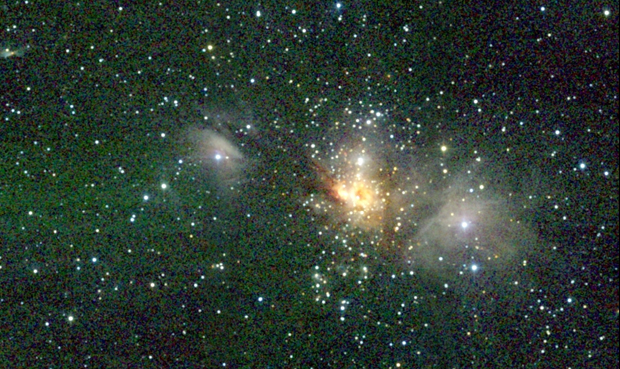
\includegraphics[scale=0.5]{MONR2A.JPG}
\caption{The molecular cloud and embedded star cluster Monoceros R2.}
\end{figure} 
\marginnote{\cite{Mon}}

The star, known as [CMD97]-1031, is located 3,400 light-years away in Monoceros. 
It is an X-ray-emitting young stellar object (YSO) with an accretion disk, a 
swirling structure of gas and dust feeding material onto the star. Despite this, it exhibits 
little mid-infrared emission, indicating a relative lack of dust in its outer regions.

{\Large A Star That Nearly Vanished}

Using data from the **Zwicky Transient Facility (ZTF), ATLAS, and Gaia, astronomers tracked the 
star’s brightness from 2014 to 2022. Normally, [CMD97]-1031 shines at magnitude 18 (r-band),
 but at the height of this event, its brightness dropped by a factor of 10, rendering it nearly invisible.

Adding to the mystery, the star “blinked” during its dimming phase, with fluctuations of **up to 2 magnitudes
before settling at a lower brightness. Once it began to recover, it remained slightly fainter and redder
than before—suggesting lasting changes in its surrounding material.

{\Large What Could Be Happening?}

Brightness variations are common in YSOs, but such a deep, prolonged dimming is rare. A similar 
event was observed in ASASSN-21qj, but its exact cause remains uncertain.

One possibility is that a dense dust cloud temporarily obscured the star, a phenomenon 
seen in UX Orionis-type variables, where orbiting dust periodically blocks starlight. 
If confirmed, this event could provide valuable insight into how dust and gas distribute a
round young stars—a crucial factor in planet formation.

{\Large Why Does This Matter?}

The fading and recovery of [CMD97]-1031 is among the most extreme cases of YSO variability observed. 
These events highlight the importance of long-term sky surveys** in uncovering hidden 
astrophysical processes that shape stars and planetary systems.

What other secrets might this young star still be hiding?\\
\hfill \textit{Word count 247}

\vspace{5cm}

\qpart
\qsubpart
In the article they talk about the median and standard deviations of the cyan and orange bands using formulae
\[ \sigma_{c-o} = \sqrt{\sigma_c^{2}+\rb{C} + \sigma^2\rb{o}}\]

so to make it more accessible I simply said the star was fainter and redder.

\qsubpart

I had to use my knowledge of how young stars are created in the presence of a molecular cloud. To try and understand
how the accretion disc would be formed around new young stars.

\end{question}




\end{document}